\section{The algorithm} \label{sec:algorithm}

\subsection{Overview} \label{sec:algorithm:overview}
The Omicron algorithm is developed in C++ and the code lives in the Virgo software repository~\cite{VirgoSVN}. Omicron relies on GWOLLUM~\cite{GWOLLUM} libraries used to perform every step of an Omicron analysis. The GWOLLUM package depends on external libraries. The FrameL~\cite{FrameL} library is used to perform IO operations on data frame files~\footnote{The frame format was developed for interferometric gravitational-wave detectors' data.}. Mathematical routines developed in the GNU Scientific Library~\cite{GSL} are commonly used by GWOLLUM functions. Discrete Fourier transforms are performed using the FFTW~\cite{FFTW} algorithm. Finally, the GWOLLUM and Omicron code heavily rely on C++ classes developed in the ROOT~\cite{Brun:1997pa} framework. For example, ROOT classes are used for plotting purposes, for event storage or for data access. To deal with package dependencies, the CMT~\cite{CMT} configuration management tool was chosen.

A fully object-oriented framework is adopted when developing GWOLLUM and Omicron, in which C++ classes and inheritance features are extensively used. The Omicron algorithm is entirely based on the \texttt{Omicron} C++ class which member functions are used to perform the analysis steps. A typical Omicron application can be represented by the sequence of functions represented in Fig.~\ref{fig:omicron_incl}. The \texttt{Omicron} constructor must be called using an input option file listing all the parameters defining the search one wants to perform. Then, the Omicron oject must be provided with time segments to process. This is done with the \texttt{Omicron::InitSegment()} function. These time segments are processed sequencially with the \texttt{Omicron::NewChunk()} function.



\begin{figure}
  \center
  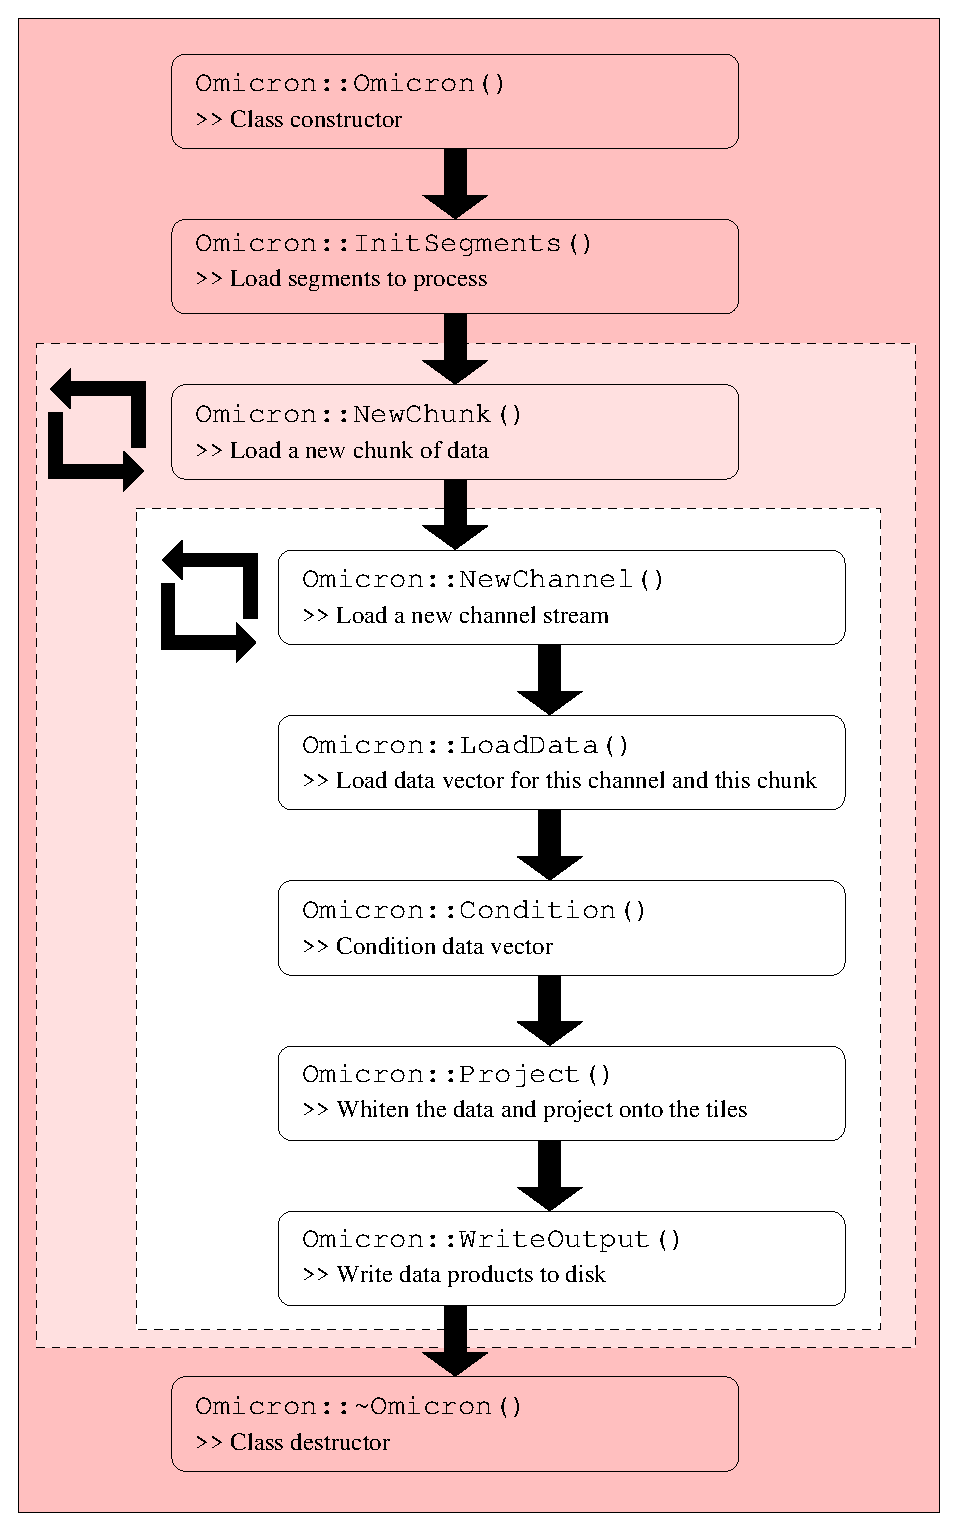
\epsfig{width=10cm, file=./figures/omicron_flowchart.eps}
  \caption{Omicron flowchart.}
  \label{fig:omicron_flowchart}
\end{figure}

\begin{figure}
  \center
  \includegraphics[angle=90, scale=0.4]{./figures/omicron_incl}
  \caption{Diagram presenting the Omicron code dependencies. Header files starting with a ``O'' are part of the Omicron Package. Header files starting with a ``T'' are taken from the ROOT~\cite{Brun:1997pa} libraries. \bluenote{Clean this!}}
  \label{fig:omicron_incl}
\end{figure}




\subsection{The data access} \label{sec:algorithm:data}
The input data time series are read using the frame library. The Omicron algorithm

\begin{figure}
  \center
  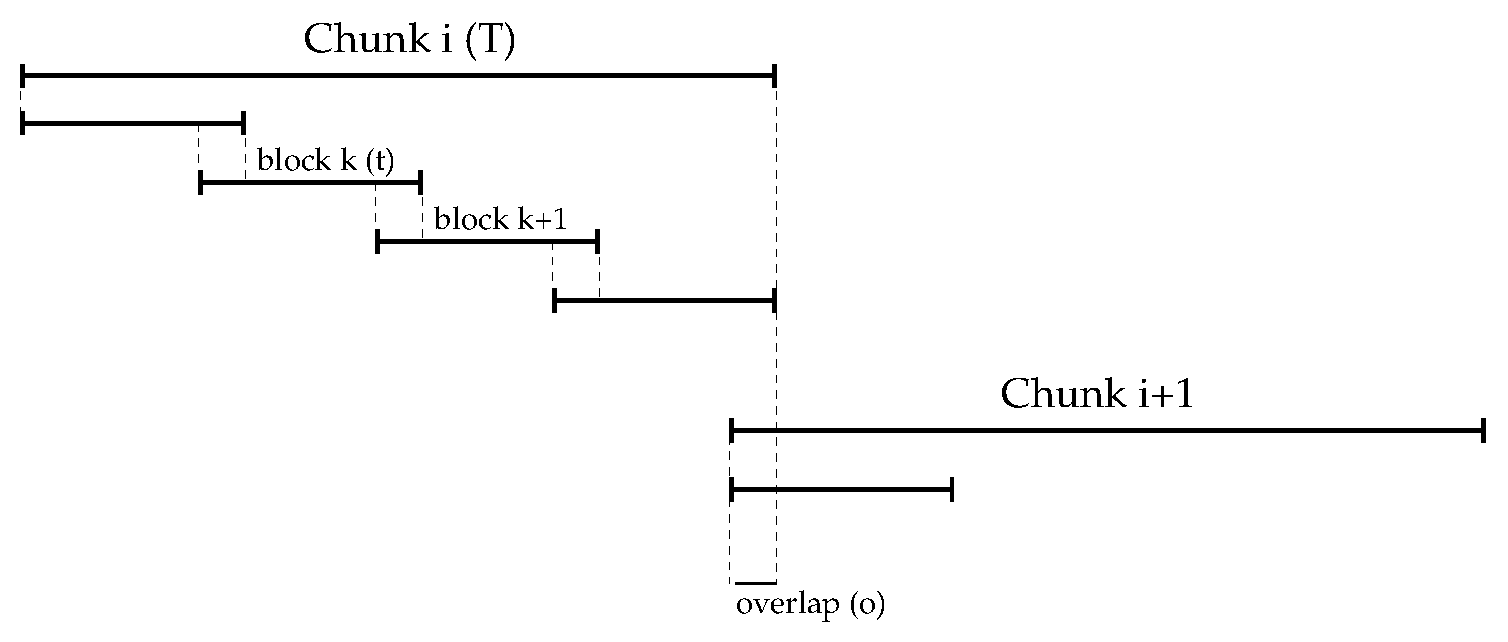
\epsfig{width=15cm, file=./figures/segmentation.eps}
  \caption{Data segmentation. The data are loaded by chunks and chunks are divided in blocks. The chunks have a duration $T$ and are used to estimate the power spectral density. The blocks have a duration $t$ and are analyzed sequentially. Chunks (and blocks) overlap with a duration $o$. This segmentation must therefore verify $T=n(t-o)+o$ where $n$ is an integer.}
  \label{fig:segmentation}
\end{figure}

\subsection{The power spectral density} \label{sec:algorithm:psd}
- PSD definition - PSD implementation (size, FT...).

To obtain a reliable PSD estimation, we use the procedure defined in~\cite{psd}.
The data chunk is divided into N segments overlapping by half, as represented in Fig.~\ref{fig:mmm}. The PSD of each segment is computed. This set of PSDs is divided into two groups corresponding to non-overlapping segments: the 'odd' (resp. 'even') group is defined with segments with an odd (resp. even) index.
\begin{figure}
  \center
  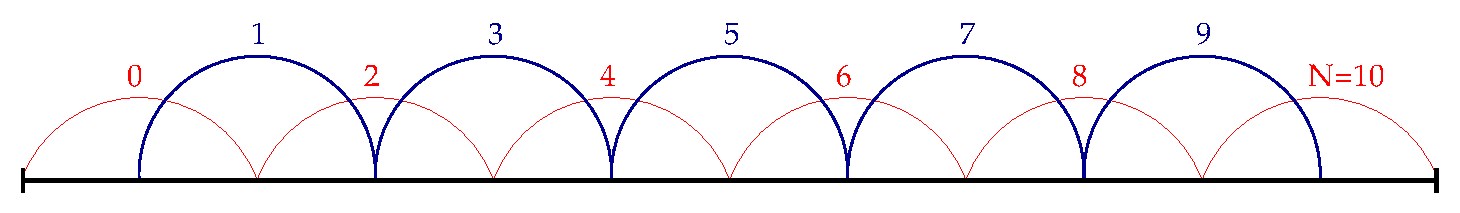
\epsfig{width=15cm, file=./figures/mmm.eps}
  \caption{Power spectral density estimation. The data chunk is divided into.}
  \label{fig:mmm}
\end{figure}

\subsection{The data conditioning} \label{sec:algorithm:conditioning}

\subsection{The tiling} \label{sec:algorithm:tiling}

\subsection{The filtering} \label{sec:algorithm:conditioning}

\subsection{The triggering} \label{sec:algorithm:triggering}

\subsection{The clustering} \label{sec:algorithm:conditioning}

\subsection{The mapping} \label{sec:algorithm:mapping}
